\newpage
\section{ Описание обратной связи по току }
Согласно требованиям задачи необходимо обеспечить скорости переброски системы не менее
$ \dot{q}_{max} = 1.73$ рад/c, при выбранном на этапе энергетического расчета передаточном
отношении редуктора $ i{gb} = 225 $. Отсюда очевидно, что минимальное время импульса управления:

$$
    T_{ctrl} = \frac{ 2 \cdot \pi }{ \dot{q}_{max} \cdot i_{gb} \cdot N_{r} \cdot p_{sm} \cdot 2 }
$$
$$
    T_{ctrl} = \frac{ 2 \cdot \pi }{ 1.73 \cdot 225 \cdot 50 \cdot 2 \cdot 2 } = 8.07 \cdot 10^{-05}
$$

Что на 2 порядка отличается от электрической постоянной времени фазы $( \simeq2 \cdot 10^{-3} )$.
Для обеспечения максимально возможного момента на скоростях близких к максимальной необходимо
быстрое нарастание тока, как было доказано ранее (\ref{ current_grow_estimate }), время роста можно
уменьшить, если увеличить напряжение.

\subsection{ Описание аппаратной части реализации токовой обратной связи }

\subsubsection{ Схематика аппаратной части }

\begin{figure}[h!]
\centering
\includegraphics[width=\textwidth, keepaspectratio, clip=true, trim=0mm 25mm 0mm 25mm]{./src/pictures/current_measuring_sheme}
\caption{Электрическая схема датчика тока}
\label{graph_speed_and_angle_comutation}
\end{figure}

Датчик тока на плате управления, выполнен на измерительном резисторе, последовательно
включенном в цепь каждой фазы. Так как управление происходит ШИМ сигналом, то стоит 4
датчика тока в кажом канале (A, B, C, D).
Сигнал с сериесного резистора через RC фильтр на измерительном резисторе и паралельно включенном
конденсаторе поступает на усилитель постоянного тока с форсирующим звеном на входе для поступает на ацп.
Передаточная функция фильтра:

$$
    \frac{ U_{out} }{ i_{pl} } = \frac{ R_{53} }{ s R_{53} C_{59} + 1 }
$$

С полосой пропускания при указанных параметрах в 100 ГГц.

\subsubsection{ Аналого-цифровое преобразование }
В нашем распоряжении 12 разрядный Аналого Цифровой Преобразователь (далее АЦП) с 16
мультиплексироваными вводами.
Имеет 2 канала измерения, которые могут использоваться как одновременно так, и последовательно.

\subsubsection{ Методика оценки зашумленности сигналов с АЦП }

\endinput

